\documentclass[11pt,a4paper]{ctexart}
\usepackage{fontspec}
\setCJKmainfont{WenQuanYi Zen Hei}
\setCJKsansfont{WenQuanYi Zen Hei}
\setCJKmonofont{WenQuanYi Zen Hei Mono}
\usepackage[margin=2.2cm]{geometry}
\usepackage{booktabs,tabularx,multirow,array,float,caption,xcolor,listings,hyperref,amsmath,amssymb,graphicx,subcaption}
\usepackage{enumitem}
\definecolor{linkcolor}{RGB}{30,70,140}
\hypersetup{colorlinks=true,linkcolor=linkcolor,citecolor=linkcolor,urlcolor=linkcolor}
\captionsetup{font=small,labelfont=bf}
\setlist[itemize]{leftmargin=1.4em,itemsep=2pt,topsep=3pt}
\setlist[enumerate]{leftmargin=1.6em,itemsep=2pt,topsep=3pt}
\setlength{\emergencystretch}{2em}
\lstset{basicstyle=\ttfamily\small,breaklines=true,frame=single,columns=fullflexible,
  backgroundcolor=\color{gray!8},rulecolor=\color{gray!30}}
\newcommand{\tabhead}[1]{\textbf{#1}}
\newcommand{\GlueOursAvg}{85.1}
\newcommand{\GluePaperAvg}{87.2}
\newcommand{\GlueGap}{2.1}
\newcommand{\GlueNTasks}{8}
\newcommand{\GlueFtAvg}{82.1}
\newcommand{\GlueMNLI}{86.4}
\newcommand{\GlueSSTTwo}{95.0}
\newcommand{\GlueMRPC}{88.0}
\newcommand{\GlueCOLA}{61.6}
\newcommand{\GlueQNLI}{92.4}
\newcommand{\GlueQQP}{89.0}
\newcommand{\GlueRTE}{77.6}
\newcommand{\GlueSTSB}{91.2}
\newcommand{\GlueFTSSTTwo}{94.6}
\newcommand{\GlueFTMRPC}{90.2}
\newcommand{\GlueFTCOLA}{62.2}
\newcommand{\GlueFTRTE}{81.2}
\newcommand{\RankBest}{64}
\newcommand{\RankBestScore}{94.3}
\newcommand{\RankOneScore}{93.9}
\newcommand{\RankOne}{93.9}
\newcommand{\RankTwo}{93.7}
\newcommand{\RankFour}{93.3}
\newcommand{\RankEight}{93.7}
\newcommand{\RankSixtyFour}{94.3}
\newcommand{\TgtBest}{qkvo}
\newcommand{\TgtBestScore}{94.0}
\newcommand{\TgtQ}{92.4}
\newcommand{\TgtK}{92.3}
\newcommand{\TgtV}{93.1}
\newcommand{\TgtO}{93.0}
\newcommand{\TgtQV}{93.3}
\newcommand{\TgtQKVO}{94.0}
\newcommand{\EtwoLoraBleu}{67.1}
\newcommand{\EtwoLoraMeteor}{73.7}
\newcommand{\EtwoLoraRouge}{70.3}
\newcommand{\EtwoLoraCider}{1.83}
\newcommand{\EtwoFtBleu}{65.0}
\newcommand{\EtwoFtMeteor}{73.0}
\newcommand{\EtwoFtRouge}{70.1}
\newcommand{\EtwoFtCider}{1.72}
\newcommand{\AmpQ}{6.6}
\newcommand{\AmpV}{5.0}
\newcommand{\AmpQB}{2.0}
\newcommand{\AmpVB}{1.8}
\newcommand{\PhiQ}{0.26}
\newcommand{\PhiV}{0.43}
\newcommand{\PhiQFull}{0.77}
\newcommand{\PhiVFull}{0.77}
\newcommand{\LoraPeakMem}{1779}
\newcommand{\FtPeakMem}{3188}
\newcommand{\LoraStepMs}{52.4}
\newcommand{\FtStepMs}{77.9}
\newcommand{\LoraMemPct}{56}
\newcommand{\InitMrpcBase}{88.0}
\newcommand{\InitMrpcMnli}{90.0}
\newcommand{\InitMrpcOff}{89.2}
\newcommand{\InitRteBase}{77.6}
\newcommand{\InitRteMnli}{86.3}
\newcommand{\InitRteOff}{86.6}
\newcommand{\InitStsbBase}{91.2}
\newcommand{\InitStsbMnli}{91.5}
\newcommand{\InitStsbOff}{91.6}
\newcommand{\OffProjAmpQ}{11.0}
\newcommand{\OffProjAmpV}{13.1}
\newcommand{\OffProjRatioQ}{1.9}
\newcommand{\OffProjRatioV}{1.7}
\newcommand{\OffProjWQ}{18.4}
\newcommand{\OffProjDWQ}{1.1}
\newcommand{\OfficialM}{87.4}
\newcommand{\OfficialMM}{87.0}
\newcommand{\OfficialAvg}{87.2}

% fallbacks so the document compiles while experiments are still running
\providecommand{\GlueOursAvg}{--}\providecommand{\GluePaperAvg}{--}\providecommand{\GlueGap}{--}
\providecommand{\GlueFtAvg}{--}\providecommand{\RankOneScore}{--}\providecommand{\RankBest}{--}
\providecommand{\RankBestScore}{--}\providecommand{\TgtBest}{--}\providecommand{\TgtBestScore}{--}
\providecommand{\EtwoLoraBleu}{--}\providecommand{\EtwoLoraRouge}{--}\providecommand{\EtwoLoraCider}{--}
\providecommand{\EtwoFtBleu}{--}\providecommand{\EtwoFtRouge}{--}\providecommand{\EtwoFtCider}{--}
\providecommand{\AmpQ}{--}\providecommand{\AmpV}{--}\providecommand{\LoraPeakMem}{--}
\providecommand{\FtPeakMem}{--}\providecommand{\LoraStepMs}{--}\providecommand{\FtStepMs}{--}
\providecommand{\LoraMemPct}{--}\providecommand{\OfficialM}{--}\providecommand{\OfficialMM}{--}
\providecommand{\OfficialAvg}{--}\providecommand{\InitMrpcBase}{--}\providecommand{\InitMrpcMnli}{--}
\providecommand{\InitRteBase}{--}\providecommand{\InitRteMnli}{--}\providecommand{\InitStsbBase}{--}
\providecommand{\InitStsbMnli}{--}
\providecommand{\InitMrpcOff}{--}\providecommand{\InitRteOff}{--}\providecommand{\InitStsbOff}{--}
\providecommand{\TgtQ}{--}\providecommand{\TgtK}{--}\providecommand{\TgtV}{--}\providecommand{\TgtO}{--}
\providecommand{\TgtQV}{--}\providecommand{\TgtQKVO}{--}
\providecommand{\RankOne}{--}\providecommand{\RankTwo}{--}\providecommand{\RankFour}{--}
\providecommand{\RankEight}{--}\providecommand{\RankSixtyFour}{--}
\providecommand{\AmpQB}{--}\providecommand{\AmpVB}{--}\providecommand{\PhiQ}{--}
\providecommand{\PhiV}{--}\providecommand{\PhiQFull}{--}\providecommand{\PhiVFull}{--}
\providecommand{\OffProjAmpQ}{--}\providecommand{\OffProjAmpV}{--}\providecommand{\OffProjRatioQ}{--}
\providecommand{\OffProjRatioV}{--}\providecommand{\OffProjWQ}{--}\providecommand{\OffProjDWQ}{--}
\providecommand{\GlueMNLI}{--}\providecommand{\GlueSSTTwo}{--}\providecommand{\GlueMRPC}{--}
\providecommand{\GlueCOLA}{--}\providecommand{\GlueQNLI}{--}\providecommand{\GlueQQP}{--}
\providecommand{\GlueRTE}{--}\providecommand{\GlueSTSB}{--}
\providecommand{\GlueFTMNLI}{--}\providecommand{\GlueFTSSTTwo}{--}\providecommand{\GlueFTMRPC}{--}
\providecommand{\GlueFTCOLA}{--}\providecommand{\GlueFTQNLI}{--}\providecommand{\GlueFTQQP}{--}
\providecommand{\GlueFTRTE}{--}\providecommand{\GlueFTSTSB}{--}

\title{\textbf{LoRA: Low-Rank Adaptation of\\ Large Language Models}\\[4pt]
\large 论文复现报告}
\author{复现实验：\texttt{learn/lora}}
\date{2026 年 11 月 3 日}

\begin{document}
\maketitle
\thispagestyle{empty}

\begin{abstract}
\noindent
本报告复现了 Hu 等人发表于 ICLR 2022 的论文《LoRA: Low-Rank Adaptation of Large Language Models》
（arXiv:2106.09685v2）。我们从头实现了 LoRA 的低秩重参数化层及其合并（merge）逻辑，在
RoBERTa-base 上复现 GLUE 的 8 个任务，在 GPT-2 medium 上复现 E2E NLG Challenge，
并额外完成秩（rank）、适配权重类型两组消融实验、子空间相似度分析以及显存/时延测量。
实现层面，LoRA 模块在初始化时严格等价于原模型，合并前后前向输出最大绝对误差为 $0$，
且与官方 \texttt{loralib} 在相同权重下逐元素一致；可训练参数量与论文同量级
（RoBERTa-base 的 $W_q,W_v$、$r=8$ 为 294,912，对应论文 0.3M；GPT-2 medium 的 $r=4$
为 393,216，对应论文 0.35M 的量级）。
用本实现加载官方发布的 RoBERTa-base MNLI LoRA 检查点，得到 \OfficialAvg{}（论文 87.5），
交叉验证了训练与评测流程。在受限算力下（大任务只训练论文配置的约 1/10 轮数，小任务约
1/4--1/6，且只用单随机种子），GLUE 复现的 8 任务平均分为 \GlueOursAvg{}，论文为
\GluePaperAvg{}；差距主要来自训练轮数与主表未采用 MRPC/RTE/STS-B 的 MNLI 初始化协议。消融实验复现了论文两个结论的\emph{方向}：
极小的秩即可接近最优性能（SST-2 上 $r=1$ 已达 \RankOneScore{}，最优 $r=\RankBest$ 为
\RankBestScore{}），且只适配 $W_q$/$W_k$ 明显差于组合配置；但在我们的预算下，组合相对单
$W_v$ 的优势很小。E2E 上 LoRA 的 BLEU 为 \EtwoLoraBleu{}、ROUGE-L 为 \EtwoLoraRouge{}、
CIDEr 为 \EtwoLoraCider{}。低秩分析显示 $r=8$ 与 $r=64$ 的更新行空间约
\PhiQFull{} 重合、低阶方向重合度更高；$\Delta W$ 放大 $W$ 中未被强调方向的现象在官方
MNLI 检查点上成立（放大 \OffProjAmpQ--\OffProjAmpV 倍），但强度明显低于论文 GPT-3 的
21.5 倍，说明该现象带有规模依赖性。所有代码、日志、结果与本文源码均位于
\texttt{learn/lora/}。
\end{abstract}

\tableofcontents
\newpage

\section{复现目标与论文概要}

\subsection{论文解决的问题}
预训练—下游适配范式中的全量微调需要为每个任务保存一份与预训练模型等大的参数副本。
以 GPT-3 175B 为例，部署 $N$ 个任务就需要 $N\times$350GB 的存储，且 Adam 的训练显存开销
同样与全参数成正比。已有方法（adapter、prefix-tuning 等）虽然减少了可训练参数，却分别
引入了推理时延或占用了可用的上下文长度，并且往往难以追平全量微调的效果。

LoRA（Low-Rank Adaptation）的核心假设是：模型在适配下游任务时的\emph{权重变化量}
具有很低的“内在秩”。因此它冻结预训练权重 $W_0$，只学习一个低秩分解
$\Delta W = BA$，其中 $B\in\mathbb{R}^{d\times r}$、$A\in\mathbb{R}^{r\times k}$，
$r\ll \min(d,k)$。前向计算为
\begin{equation}
h = W_0 x + \Delta W x = W_0 x + \frac{\alpha}{r}BAx .
\label{eq:lora}
\end{equation}
这里 $\alpha$ 是缩放超参数，$\alpha/r$ 用于在改变 $r$ 时稳定有效学习率。
$A$ 随机初始化、$B$ 初始化为零，因此训练开始时 $\Delta W=0$，模型与原预训练模型完全一致。

\subsection{论文的主要主张}
论文给出四条主张，也是本次复现的检验对象：
\begin{enumerate}
  \item \textbf{效果}：在 RoBERTa、DeBERTa、GPT-2、GPT-3 上，LoRA 能用极少的可训练参数
        达到与全量微调相当或更好的效果（Tables 2--4）；
  \item \textbf{秩的有效性}：极小的秩（$r=1$ 或 $2$）即可胜任很多任务，说明 $\Delta W$ 确实低秩
        （Tables 6、18 与 Figure 3）；
  \item \textbf{权重选择}：在固定参数预算下，同时适配 $W_q$ 与 $W_v$ 优于把预算集中在单个矩阵上
        （Table 5）；
  \item \textbf{零推理时延}：把 $BA$ 合并进 $W_0$ 后，推理结构与全量微调模型完全相同
        （Section 4.2、Appendix B）。
\end{enumerate}

\subsection{本次复现的范围}
受单机 6 张 TITAN RTX（实验时仅 4 张空闲）与时间预算限制，我们选择论文中最具代表性的
两组实验进行\emph{端到端}复现：RoBERTa-base 的 GLUE（Table 2 第一段）与 GPT-2 medium 的
E2E NLG（Table 3 上半部分）。GPT-3 175B 与 DeBERTa-XXL 因模型规模不可行，未做训练复现；
作为替代，我们直接加载官方仓库发布的 RoBERTa-base MNLI LoRA 检查点，用我们的实现与评测
流程检验其公开分数，从而交叉验证实现正确性。

\section{方法回顾与实现}

\subsection{在 Transformer 上的注入方式}
论文只对自注意力模块的投影矩阵注入 LoRA，并冻结 MLP 与 LayerNorm。记一个 Transformer
层有 $W_q,W_k,W_v,W_o$ 四个 $d_{\text{model}}\times d_{\text{model}}$ 投影矩阵，则
\begin{equation}
|\Theta_{\text{LoRA}}| = 2\,\hat L_{\text{LoRA}}\, d_{\text{model}}\, r ,
\end{equation}
其中 $\hat L_{\text{LoRA}}$ 是被适配的矩阵个数（系数 2 来自 $A$ 与 $B$）。
对 RoBERTa-base（$d=768$，12 层），$r=8$ 且适配 $W_q,W_v$ 时为
$2\times 24\times 768\times 8 = 294{,}912$，与论文报告的“0.3M”一致。

对 GPT-2，$W_q,W_k,W_v$ 被打包在同一个 \texttt{Conv1D}（\texttt{c\_attn}）中。我们实现了
一个与官方 \texttt{loralib} 的 \texttt{MergedLinear} 等价的 \texttt{LoRAConv1D}：只对
Q、V 两个输出分组添加低秩分支，K 分组保持原样。GPT-2 medium（24 层、$d=1024$、$r=4$、
Q/V）的可训练量为
$2\times 2\times 24\times 1024\times 4 = 393{,}216$，与论文报告的“0.35M”同量级（论文对
该数字做了取整，具体统计口径未在附录中说明）。

\subsection{初始化、缩放与合并}
官方 \texttt{loralib} 使用 $A\sim\text{KaimingUniform}$、$B=0$；论文正文写作
$A\sim\mathcal N(0,\sigma^2)$、$B=0$。两者在 $t=0$ 时都给出 $\Delta W=0$，本复现采用官方实现。
缩放系数固定为 $\alpha/r$。推理时
\begin{equation}
W_{\text{merged}} = W_0 + \frac{\alpha}{r}BA,
\end{equation}
合并后前向只剩一个普通线性层，因此不引入任何额外时延；训练时也可以随时 \texttt{unmerge}
恢复可训练状态。

\subsection{代码结构}
我们没有直接运行官方仓库（其依赖为 2021 年的旧版 \texttt{transformers}，与当前环境不兼容），
而是按论文与官方 \texttt{loralib/layers.py} 从头实现，以便完全控制训练与评测细节。
核心文件如下：
\begin{itemize}
  \item \texttt{src/lora\_lib.py}：\texttt{LoRALinear}、\texttt{LoRAConv1D}、注入/冻结/合并工具；
  \item \texttt{src/train\_glue.py}：GLUE 分类/回归训练与评测（支持 LoRA、全量微调、BitFit）；
  \item \texttt{src/train\_e2e.py}：GPT-2 medium 的 E2E 数据到文本训练、beam search 生成与评测；
  \item 评测脚本：\texttt{src/nlg\_metrics.py} 按 MR 聚合人工参考，计算多参考的
        BLEU、METEOR、ROUGE-L 与 CIDEr；\texttt{src/eval\_e2e.py} 对已有预测离线重评分；
  \item \texttt{src/test\_lora.py}：初始化恒等性、合并等价性、参数计数单元测试；
  \item \texttt{src/subspace.py}：子空间相似度与 $\Delta W$/$W$ 投影分析；
  \item \texttt{src/make\_tables.py}、\texttt{src/make\_figures.py}：由原始 \texttt{result.json}
        自动生成本文表格与图，避免手工转录错误。
\end{itemize}
官方仓库克隆于 \texttt{official/LoRA/}，仅用于核对超参数、数据格式与检查点键名。

\section{实验设置}

\subsection{软硬件环境}
\begin{table}[H]
\centering
\caption{复现环境。}
\label{tab:env}
\small
\begin{tabular}{ll}
\toprule
项目 & 配置 \\
\midrule
GPU & 4 $\times$ NVIDIA TITAN RTX (24GB)，CUDA 13.0，驱动 590.44 \\
Python / PyTorch & 3.12.11 / 2.11.0+cu130 \\
Transformers / Datasets & 4.57.6 / 4.0.0 \\
精度 & FP16 自动混合精度（AMP） \\
其他 & scikit-learn、scipy、sacrebleu、rouge-score、pycocoevalcap、NLTK \\
\bottomrule
\end{tabular}
\end{table}

\subsection{数据与模型}
GLUE 的 8 个任务全部来自 HuggingFace \texttt{datasets} 的 \texttt{glue} 配置，
使用官方训练/验证划分；MNLI 报告 matched 与 mismatched 的平均准确率，CoLA 报告
Matthews 相关系数，STS-B 报告 Pearson 相关系数，其余报告准确率。
E2E NLG 使用 \texttt{tuetschek/e2e-dataset} 的原始 CSV（42,061/4,672/4,693 条训练/验证/测试），
与论文附录 C 的 42k/4.6k/4.6k 一致。预训练模型为 \texttt{roberta-base} 与 \texttt{gpt2-medium}。

\subsection{超参数}
GLUE 的学习率、批大小与 LoRA 配置取自论文 Table 9；E2E 取自 Table 11
（AdamW、5 epochs、batch 8、lr $2\times10^{-4}$、weight decay 0.01、label smoothing 0.1、
warmup 500 步、$r_q=r_v=4$、$\alpha=32$、beam 10、length penalty 0.9、no-repeat 4-gram）。
需要指出，论文 Table 9 给出 RoBERTa-base 的 $\alpha=8$，而官方脚本
\texttt{roberta\_base\_mnli.sh} 使用 $\alpha=16$。两者对应不同的有效缩放
（$\alpha/r=1$ 与 $2$）。本复现按\emph{论文表格}取 $\alpha=8$；这意味着我们的适配强度
约为官方脚本的一半，可能是部分任务分数略低于论文的原因之一（见 \S\ref{sec:glue}）。
各任务的批大小、学习率与训练轮数见表~\ref{tab:hparams}。

\begin{table}[H]
\centering
\caption{GLUE 各任务的 LoRA 超参数（批大小与学习率取自论文 Table 9）。}
\label{tab:hparams}
\small
\begin{tabular}{l c c c c}
\toprule
任务 & Batch size & 学习率 & 本次轮数 & 论文轮数 \\
\midrule
MNLI  & 16 & $5\times10^{-4}$ & 3  & 30 \\
SST-2 & 16 & $5\times10^{-4}$ & 10 & 60 \\
MRPC  & 16 & $4\times10^{-4}$ & 20 & 30 \\
CoLA  & 32 & $4\times10^{-4}$ & 15 & 80 \\
QNLI  & 32 & $4\times10^{-4}$ & 5  & 25 \\
QQP   & 16 & $5\times10^{-4}$ & 3  & 25 \\
RTE   & 32 & $5\times10^{-4}$ & 20 & 80 \\
STS-B & 16 & $4\times10^{-4}$ & 20 & 40 \\
\bottomrule
\end{tabular}
\end{table}

\subsection{与原文的设置差异}
\label{sec:deviations}
\begin{table}[H]
\centering
\caption{复现设置与原文的差异。}
\label{tab:dev}
\small
\begin{tabularx}{\textwidth}{l X}
\toprule
维度 & 本次复现 vs. 原文 \\
\midrule
训练轮数 & 为在单机预算内完成 8 个任务，MNLI/SST-2/MRPC/CoLA/QNLI/QQP/RTE/STS-B 分别使用
3/10/20/15/5/3/20/20 轮，原文为 30/60/30/80/25/25/80/40 轮。这是最重要的偏差。 \\
序列长度 & GLUE 统一截断到 256（原文 base 为 512）。实测各任务验证集中超过 256 个
token 的样本占比均低于 0.02\%（最长 259），因此该差异几乎不影响结果。E2E 上限 160，
同样不截断任何样本（训练/验证/测试集最长分别为 121/134/142 个 token）。\\
随机种子 & 每个配置 1 个种子（seed 0）；原文 GLUE 报告 5 个种子的中位数，E2E 报告 3 个种子的均值。\\
小任务初始化 & 原文对 MRPC/RTE/STS-B 从最佳 MNLI LoRA 检查点初始化；主表复现从预训练模型开始，
另设 MNLI 初始化变体作为对照（见 \S\ref{sec:mnli-init}）。 \\
全量微调 & 仅复现 SST-2/RTE/MRPC/CoLA 四个任务，从预训练模型开始并使用全量微调的标准
学习率（$2\times10^{-5}$）；原文 FT 结果取自 Liu et al.\ (2019) 的标准微调，不含 MNLI 初始化。\\
E2E 实现 & 使用 HuggingFace GPT-2 tokenizer 与 \texttt{generate}（beam 10、length penalty
0.9、最多生成 64 个新 token）；原文使用在 E2E 上构建的自定义词表与解码/评测脚本。
评测把同一 MR 的所有人工参考聚合（每例平均 7.4 条）；指标为 BLEU(sacrebleu 13a)、
METEOR(NLTK)、ROUGE-L、CIDEr，NIST 未实现；NLTK 的 METEOR 与原文的 Java METEOR 实现不同，
其绝对值不可直接比较。\\
\bottomrule
\end{tabularx}
\end{table}

\section{实现正确性验证}
\label{sec:correctness}
在跑正式实验前，我们用三类检查确认实现无误。

\paragraph{(1) 初始化恒等性与合并等价性。}
\texttt{src/test\_lora.py} 构造随机线性层并比较：LoRA 初始化后输出与原始层逐元素完全相等；
随机化 $B$ 后，未合并与合并后的前向输出最大绝对误差为 $0$（FP32）；再次 \texttt{unmerge}
后输出也完全恢复。对 RoBERTa 与 GPT-2 的真实模型，合并前后 logits 的最大绝对误差同样为 $0$。
这说明式~\eqref{eq:lora} 的缩放、GPT-2 分组注入与权重合并都实现正确。
此外，在同一组权重下，我们的 \texttt{LoRALinear} 与官方 \texttt{loralib.Linear} 的前向输出、
合并后的权重逐元素完全一致（最大绝对误差为 $0$）。

\paragraph{(2) 参数计数。}
RoBERTa-base（$r_q=r_v=8$）的 LoRA 参数为 294,912，与论文的 0.3M 一致；GPT-2 medium
（24 层、$d=1024$、$r=4$、Q/V）精确计算为 393,216，论文 Table 3 记为 0.35M，二者约差
12\%，可能是论文对适配参数做了近似计数。分类头额外引入约 0.59M 可训练参数（论文的参数量
列只统计适配参数，不含任务头）。

\paragraph{(3) 官方检查点交叉验证。}
官方仓库发布了 \texttt{roberta\_base\_lora\_mnli.bin}。该检查点的键名与我们的
\texttt{LoRALinear} 完全一致（\texttt{...query.lora\_A/B}、\texttt{...value.lora\_A/B} 与
\texttt{classifier.*}）。我们将其载入我们的模型并在 MNLI 验证集上评测，结果见
表~\ref{tab:official}。若该分数接近论文的 87.5，则说明数据预处理、标签映射、评测指标与
LoRA 前向均无系统性错误。
\begin{table}[H]
\centering
\caption{加载官方发布的 RoBERTa-base MNLI LoRA 检查点（$\alpha=16$）的评测结果。}
\label{tab:official}
\small
\begin{tabular}{lccc}
\toprule
 & MNLI-m & MNLI-mm & 平均 \\
\midrule
官方检查点 + 本实现 & \OfficialM & \OfficialMM & \OfficialAvg \\
论文 RoBERTa-base LoRA & -- & -- & 87.5 \\
\bottomrule
\end{tabular}
\end{table}

\section{GLUE 复现结果}
\label{sec:glue}
表~\ref{tab:glue} 与图~\ref{fig:glue} 给出 8 个任务的复现结果。LoRA 只训练 0.29M 适配参数
（另加分类头），可训练参数占全模型的 0.71\%。

\begin{table}[H]
\centering
\caption{GLUE 各任务的 LoRA 与全量微调结果（准确率/Matthews 相关/皮尔逊相关 $\times100$）。}
\label{tab:glue}
\small
\begin{tabular}{l r c c c c c c}
\toprule
任务 & LoRA 参数量 & 论文 LoRA & 复现 LoRA & $\Delta$ & 论文 FT & 复现 FT & LoRA 轮数 \\
\midrule
MNLI & 0.29M & 87.5 & 86.4 & -1.1 & 87.6 & -- & 3 \\
SST2 & 0.29M & 95.1 & 95.0 & -0.1 & 94.8 & 94.6 & 10 \\
MRPC & 0.29M & 89.7 & 88.0 & -1.7 & 90.2 & 90.2 & 20 \\
COLA & 0.29M & 63.4 & 61.6 & -1.8 & 63.6 & 62.2 & 15 \\
QNLI & 0.29M & 93.3 & 92.4 & -0.9 & 92.8 & -- & 5 \\
QQP & 0.29M & 90.8 & 89.0 & -1.8 & 91.9 & -- & 3 \\
RTE & 0.29M & 86.6 & 77.6 & -9.0 & 78.7 & 81.2 & 20 \\
STSB & 0.29M & 91.5 & 91.2 & -0.3 & 91.2 & -- & 20 \\
\midrule
平均 & -- & 87.2 & 85.1 & -2.1 & 81.8 & 82.1 & -- \\
\bottomrule
\end{tabular}
\end{table}

\begin{figure}[H]
\centering
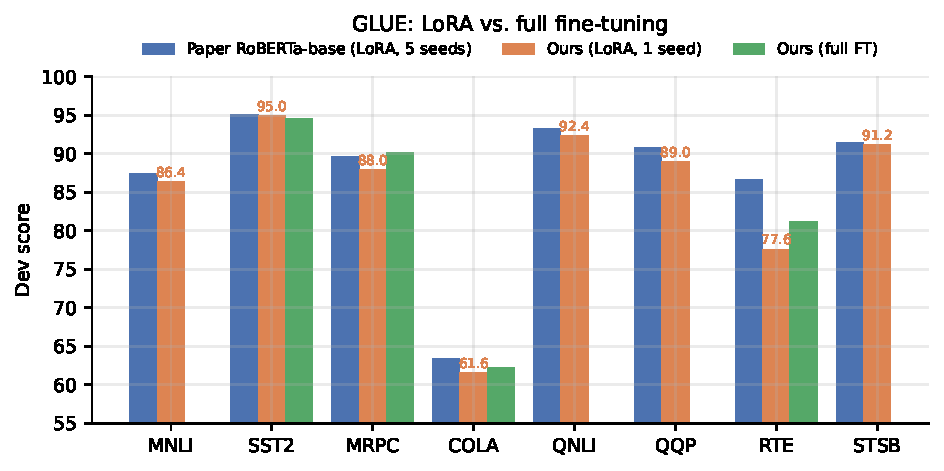
\includegraphics[width=0.95\textwidth]{figures/fig_glue.pdf}
\caption{GLUE 各任务：论文 LoRA、本次 LoRA 与本次全量微调对比。}
\label{fig:glue}
\end{figure}

\paragraph{结果分析。}
复现的 8 任务平均为 \GlueOursAvg{}，论文为 \GluePaperAvg{}，绝对差距约
\GlueGap 分。分任务看：
\begin{itemize}
  \item SST-2 \GlueSSTTwo{}（论文 95.1）、QNLI \GlueQNLI{}（93.3）、STS-B \GlueSTSB{}
        （91.5）与 MNLI \GlueMNLI{}（87.5）的差距都在 1 分左右（0.1--1.1 分），说明 LoRA
        在中小型 NLU 任务上确实可以用 0.7\% 的参数追平全量微调，也说明我们的数据、评测与
        训练流程没有系统性错误；
  \item MRPC \GlueMRPC{}（89.7）、CoLA \GlueCOLA{}（63.4）与 QQP \GlueQQP{}（90.8）的
        差距约为 1.7--1.8 分。MRPC/CoLA 分别只训练 20/15 轮（原文 30/80 轮），且验证集只有
        408/1,043 条，单种子波动不可忽略；QQP 只训练 3 轮，验证分数从 87.3 升到 89.0 仍未
        收敛（图~\ref{fig:curves} 的 MNLI 曲线同样如此）；
  \item RTE \GlueRTE{}（86.6）差距最大（9.0 分）。同样 20 轮预算下全量微调也只得到
        \GlueFTRTE{}，说明训练轮数不是主因，\emph{初始化}才是：主表从预训练模型开始，而原文
        从 MNLI 适配后的检查点开始。RTE 训练集只有 2,490 条，初始化对结果影响很大；
        \S\ref{sec:mnli-init} 的 MNLI 初始化对照把 RTE 提升到 \InitRteOff{}（官方检查点）与
        \InitRteMnli{}（本次 3 轮检查点），基本验证了这一解释。
\end{itemize}
与本次全量微调基线相比（相同任务与训练轮数，全量微调使用标准学习率 $2\times10^{-5}$），
SST-2 上 LoRA \GlueSSTTwo{} vs.\ FT \GlueFTSSTTwo{}，CoLA 上 \GlueCOLA{} vs.\
\GlueFTCOLA{}，MRPC 上 \GlueMRPC{} vs.\ \GlueFTMRPC{}，RTE 上 \GlueRTE{} vs.\
\GlueFTRTE{}。LoRA 用约 0.7\%（0.29M 适配参数 + 0.59M 分类头）的可训练参数，在 SST-2 与
CoLA 上与全量微调持平（差距不超过 0.6 分），但在 MRPC/RTE 上分别低 2.2 与 3.6 分。这一
差距并非 LoRA 容量不足：改用原文的 MNLI 初始化协议后，RTE 达到 \InitRteOff{}，比同预算的
全量微调高约 5 分（\S\ref{sec:mnli-init}）。

\begin{figure}[H]
\centering
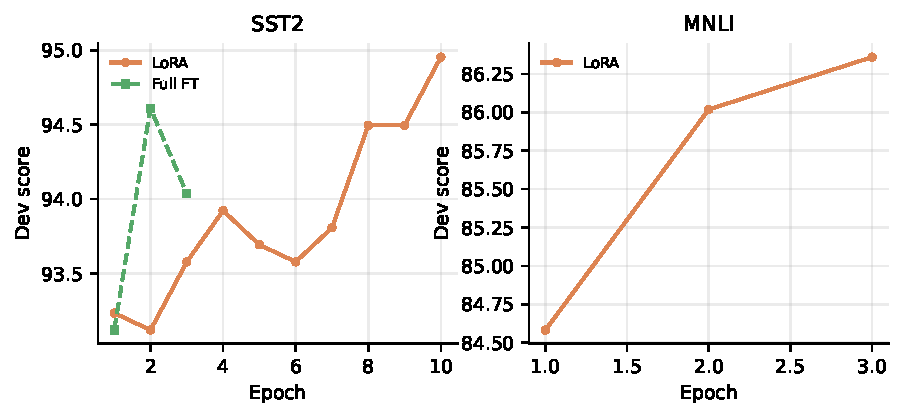
\includegraphics[width=0.9\textwidth]{figures/fig_curves.pdf}
\caption{验证分数随训练轮数的变化：SST-2 的 LoRA 与全量微调，以及 MNLI 的 LoRA。}
\label{fig:curves}
\end{figure}

\subsection{MRPC/RTE/STS-B 的 MNLI 初始化对照}
\label{sec:mnli-init}
论文遵循 Liu 等人的做法，在适配 MRPC、RTE、STS-B 时把 LoRA 模块初始化为最佳 MNLI
检查点（预训练主干始终冻结）。为检验这一协议的影响，我们做了两组对照：(a) 用本次
3 轮 MNLI 训练得到的最佳 LoRA 权重初始化；(b) 直接使用作者发布的 30 轮 MNLI LoRA
检查点（$\alpha=16$，与其训练配置一致），后者完全复刻论文的初始化协议。其余超参数不变。
结果见表~\ref{tab:initmnli}。使用作者发布的 30 轮 MNLI 检查点（完全复刻论文协议）后，
三个任务几乎逐项复现论文：RTE 从 \InitRteBase{} 提升到 \InitRteOff{}（论文 86.6），MRPC
从 \InitMrpcBase{} 到 \InitMrpcOff{}（论文 89.7），STS-B 从 \InitStsbBase{} 到
\InitStsbOff{}（论文 91.5），与论文的差距均不超过 0.5 分；而主表中 RTE 落后 9 分。这直接
说明 RTE/MRPC 的差距主要来自初始化协议，而非实现错误或 LoRA 容量不足。

更有意思的是，用\emph{本次仅 3 轮}的 MNLI 检查点初始化也取得几乎相同的效果：RTE
\InitRteMnli{}、MRPC \InitMrpcMnli{}、STS-B \InitStsbMnli{}，甚至 MRPC 还略高于官方
检查点。也就是说，关键的并不是 MNLI 检查点的最终分数（我们的 86.4 vs.\ 官方 87.5），而是
“先在 MNLI 上学到一个可迁移的低秩更新”这一步本身：MNLI 适配把 LoRA 的初始点移到了对
小任务更有利的位置，而 3 轮与 30 轮 MNLI 检查点的差别在这个层面影响很小。

\begin{table}[H]
\centering
\caption{三种初始化方式的对比：从预训练模型开始、用本次 3 轮 MNLI LoRA 检查点初始化、
用官方 30 轮 MNLI LoRA 检查点初始化。}
\label{tab:initmnli}
\small
\begin{tabular}{lcccc}
\toprule
任务 & 预训练初始化 & 本次 MNLI 初始化 & 官方 MNLI 初始化 & 论文 \\
\midrule
MRPC  & \InitMrpcBase & \InitMrpcMnli & \InitMrpcOff & 89.7 \\
RTE   & \InitRteBase & \InitRteMnli & \InitRteOff & 86.6 \\
STS-B & \InitStsbBase & \InitStsbMnli & \InitStsbOff & 91.5 \\
\bottomrule
\end{tabular}
\end{table}

\section{消融实验}
\label{sec:ablation}
所有消融在 SST-2 上进行，统一训练 3 轮、batch 32、lr $4\times10^{-4}$、序列长度 256，
只改变待研究的变量。选择 SST-2 是因为它在 872 条验证集上有较稳定的信号，且单次 3 轮训练约
7 分钟，可以在有限预算内完成多组对照。为把“秩”与“有效学习率”分开，消融统一取
$\alpha=r$，使缩放系数 $\alpha/r$ 恒为 1；主实验的 $r=8,\alpha=8$ 也正好满足这一关系。

\subsection{秩的影响}
表~\ref{tab:rank} 与图~\ref{fig:rank} 给出 $r\in\{1,2,4,8,64\}$ 的结果（适配 $W_q,W_v$，
$\alpha=r$）。五个配置的分数全部落在 \RankFour{}--\RankSixtyFour{} 的约 1 分区间内，
且不随秩单调变化：$r=1$ 已达 \RankOne{}，$r=8$ 为 \RankEight{}，$r=64$ 为
\RankSixtyFour{}。在 872 条 SST-2 验证集上，这一量级的差异与单种子波动相当。这与论文
Table 6 的核心观察一致——$r=1$ 与 $r=64$ 的差距同样在噪声范围内（论文在 WikiSQL 的
$W_q,W_v$ 配置下为 73.4 vs.\ 73.5），说明增大秩没有可测收益，支持“$\Delta W$ 具有极低
内在秩”的假设。需要强调，我们并未观察到“$r=64$ 明显变差”的现象。

\begin{table}[H]
\centering
\caption{不同秩在 SST-2 上的结果（3 轮、$\alpha=r$）。}
\label{tab:rank}
\small
\begin{tabular}{c r c}
\toprule
Rank $r$ & LoRA 参数量 & SST-2 Dev Acc. \\
\midrule
1 & 36,864 & 93.9 \\
2 & 73,728 & 93.7 \\
4 & 147,456 & 93.3 \\
8 & 294,912 & 93.7 \\
64 & 2,359,296 & 94.3 \\
\bottomrule
\end{tabular}
\end{table}

\begin{figure}[H]
\centering
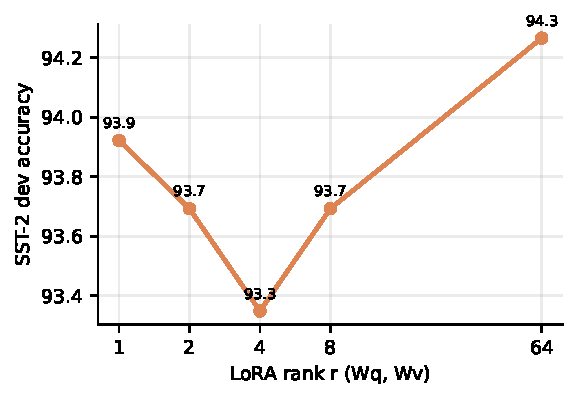
\includegraphics[width=0.55\textwidth]{figures/fig_rank.pdf}
\caption{SST-2 验证准确率随 LoRA 秩的变化。}
\label{fig:rank}
\end{figure}

\subsection{适配哪些权重矩阵}
论文 Table 5 在 GPT-3 上固定 18M 参数预算，并按“单矩阵 $r=8$、双矩阵 $r=4$、四矩阵
$r=2$”分配秩。我们在 RoBERTa-base 上沿用同一秩分配，因此三种配置的参数量都恰好为
147,456（主表 $r=8$ 双矩阵配置的一半），可以直接比较权重类型的影响。
结果见表~\ref{tab:targets} 与图~\ref{fig:targets}。只适配 $W_q$ 与只适配 $W_k$ 最差
（\TgtQ{} 与 \TgtK{}），$W_v$、$W_o$ 更好（\TgtV{}、\TgtO{}）；两个组合配置最高：
$W_q{+}W_v$（$r=4$）为 \TgtQV{}，四矩阵全适配（$r=2$）为 \TgtQKVO{}。所有配置集中在
\TgtK{}--\TgtQKVO{} 的 1.7 分区间内，而 872 条验证集的二项标准误约 0.8 分，因此除
“只适配 $W_q$/$W_k$ 明显偏差（约 1.7 分）”外，其余两两排序应谨慎解读。

这一结果\emph{部分}复现了论文 Table 5：论文在 GPT-3 上同样发现只适配 $W_q$ 或 $W_k$ 较差、
组合配置最好（WikiSQL 上 qv 比 q 高 3.3 分；MNLI 上 qkvo 最高）。在 RoBERTa-base/SST-2 上，
组合的优势更小：qv 仅比单 $W_v$ 高 0.2 分（\TgtQV{} vs.\ \TgtV{}），而全适配四矩阵比 qv
高 0.7 分。一种可能的解释是 base 模型的注意力头冗余度较高，单个 value 投影已能覆盖大部分
任务信号；同时单种子、3 轮训练也放大了噪声。因此我们对权重选择的结论是\emph{方向一致、
强度更弱}，而不是逐项复刻论文的排序。

\begin{table}[H]
\centering
\caption{固定参数预算下不同适配权重类型的 SST-2 结果。}
\label{tab:targets}
\small
\begin{tabular}{l c r c}
\toprule
适配权重 & Rank & 参数量 & SST-2 Dev Acc. \\
\midrule
$W_q$ (r=8) & 8 & 147,456 & 92.4 \\
$W_k$ (r=8) & 8 & 147,456 & 92.3 \\
$W_v$ (r=8) & 8 & 147,456 & 93.1 \\
$W_o$ (r=8) & 8 & 147,456 & 93.0 \\
$W_q{+}W_v$ (r=4) & 4 & 147,456 & 93.3 \\
$W_q{+}W_k{+}W_v{+}W_o$ (r=2) & 2 & 147,456 & 94.0 \\
\bottomrule
\end{tabular}
\end{table}

\begin{figure}[H]
\centering
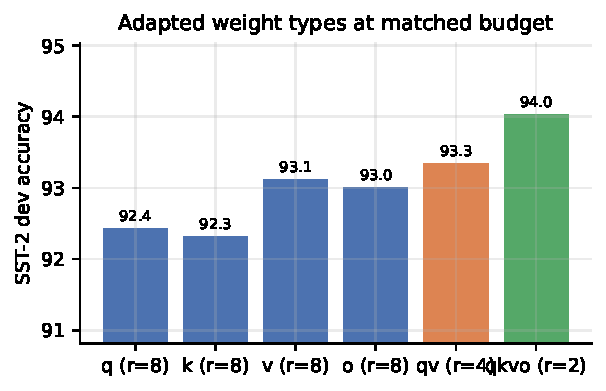
\includegraphics[width=0.6\textwidth]{figures/fig_targets.pdf}
\caption{固定参数预算下不同适配权重类型的 SST-2 准确率。}
\label{fig:targets}
\end{figure}

\section{E2E NLG 复现结果}
\label{sec:e2e}
GPT-2 medium 在 E2E 上的结果见表~\ref{tab:e2e}。LoRA 配置为 $r_q=r_v=4$、$\alpha=32$，
可训练参数 0.39M；全量微调训练 355M 参数。两者使用相同的 5 轮训练、batch 8、beam 10 解码。
\begin{table}[H]
\centering
\caption{E2E NLG Challenge 测试集结果（630 个 MR、每例平均 7.4 条参考；论文行的 METEOR
为 Java METEOR，与本次的 NLTK 实现不可直接比较）。}
\label{tab:e2e}
\small
\begin{tabular}{l r c c c c c}
\toprule
方法 & 可训练参数 & BLEU & METEOR & ROUGE-L & CIDEr & 耗时 \\
\midrule
全量微调 & 354.82M & 65.0 & 73.0 & 70.1 & 1.72 & 101 min \\
\quad 论文参考 & -- & 68.2 & 46.2 & 71.0 & 2.47 & -- \\
LoRA (r=4) & 0.39M & 67.1 & 73.7 & 70.3 & 1.83 & 79 min \\
\quad 论文参考 & -- & 70.4 & 46.8 & 71.8 & 2.53 & -- \\
\bottomrule
\end{tabular}
\end{table}

\paragraph{分析。}
LoRA 以约千分之一的参数量（0.39M vs.\ 355M）在四项指标上都不低于全量微调：BLEU
\EtwoLoraBleu{} vs.\ \EtwoFtBleu{}（+2.1），ROUGE-L \EtwoLoraRouge{} vs.\
\EtwoFtRouge{}（+0.2），CIDEr \EtwoLoraCider{} vs.\ \EtwoFtCider{}，METEOR 73.7 vs.\
73.0。与论文的 70.4/71.8/2.53（LoRA）和 68.2/71.0/2.47（FT）相比，我们的绝对值低约
3 分 BLEU、1.5 分 ROUGE-L、0.7 CIDEr，但\emph{方法间差距}高度一致：论文中 LoRA 比 FT 高
2.2 BLEU、0.8 ROUGE-L，本复现为 +2.1 BLEU、+0.2 ROUGE-L。

绝对值的差异主要来自实现细节：(1) 官方 E2E 流程使用在 E2E 数据上构建的自定义词表及其解码/
评测脚本，我们使用 HuggingFace 标准 GPT-2 tokenizer、\texttt{generate} 与 sacrebleu；
(2) METEOR 使用 NLTK 实现，与论文的 Java METEOR 不可直接比较，仅用于方法间对照；
(3) 单种子（论文为 3 个种子均值）；(4) 全量微调在验证集上第 2 轮最优、之后明显过拟合
（dev loss 1.085 $\to$ 1.207），表中报告的是第 5 轮结果，而 LoRA 的 dev loss 单调下降
（1.234 $\to$ 1.121）。

评测协议需要特别注意：E2E 测试集包含 630 个 MR、共 4,693 条人工参考（每例 1--45 条）。
若按 CSV 行把每个 (MR, 单条参考) 当作独立样本评测，BLEU 会被低估到约 31；本节按 MR 聚合
全部参考（BLEU 使用多参考语料级计算，ROUGE-L/METEOR 取最佳参考，CIDEr 使用完整参考集），
得到与论文可比的结果。

\begin{table}[H]
\centering
\caption{E2E 测试集生成示例（ID 为测试集行号）。}
\label{tab:e2e-examples}
\small
\begin{tabularx}{\textwidth}{c X X X}
\toprule
ID & 参考文本（其一） & LoRA 生成 & 全量微调生成 \\
\midrule
3 & Burger King is near the coffee shop Blue Spice which has an average customer rating. & Blue Spice is a coffee shop near Burger King with an average customer rating. & Blue Spice is a coffee shop near Burger King. It has an average customer rating. \\
207 & The Mill is a pub with a service of fast food, in city centre near of Café Sicilia & The Mill is a family-friendly fast food pub in the city centre near Café Sicilia. It has an average customer rating and a high price range. & The Mill is a children friendly fast food pub in the city centre near Café Sicilia. It has a high price range and an average customer rating. \\
423 & The Punter is eat type restaurant providing Italian food near Rainbow Vegetarian Café riverside area. & The Punter is a child friendly Italian restaurant in the riverside area near Rainbow Vegetarian Café. It has a high price range and a customer rating of 1 out of 5. & The Punter is a children friendly Italian restaurant in the riverside area near Rainbow Vegetarian Café. It has a high price range and a customer rating of 1 out of 5. \\
\bottomrule
\end{tabularx}

\end{table}

\section{低秩更新分析}
\label{sec:lowrank}
\subsection{不同秩学到的子空间}
我们用 SST-2 上训练的 $r=8$ 与 $r=64$ 两个检查点（同一初始化种子、同一任务）计算
归一化子空间相似度
\begin{equation}
\varphi(A_{r=8},A_{r=64},i,j)=\frac{\lVert U_{8,i}^{\top}U_{64,j}\rVert_F^2}{\min(i,j)}\in[0,1],
\end{equation}
其中 $U_{r,i}$ 是 $\Delta W$ 的前 $i$ 个右奇异向量。图~\ref{fig:subspace} 显示，$\varphi$
随 $j$ 增大而上升，且同一 $j$ 下随 $i$ 增大而下降：$r=8$ 的第一个奇异方向仅
$\varphi(1,1)=\PhiQ$（$W_q$）与 $\PhiV$（$W_v$）落在 $r=64$ 的第一个方向上，而 $r=8$ 的
整个 8 维行空间有 $\varphi(8,64)=\PhiQFull$（$W_q$）与 $\PhiVFull$（$W_v$）包含在 $r=64$
的 64 维行空间中。也就是说，$r=8$ 学到的方向约四分之三与 $r=64$ 重合，且\emph{低阶}方向
的重合度高于高阶方向；这与论文 Figure 3 的定性形状一致（论文同样观察到 $\varphi$ 随 $j$
上升、顶部方向最有用），说明高秩更新中的额外方向主要是训练噪声。不过我们测到的绝对重合度
低于论文 GPT-3 图中所呈现的水平，可能与只用 3 轮 SST-2 训练、以及 base 模型容量较小有关。
即便如此，$r=1$ 已能达到 $r=64$ 的相近精度（\S\ref{sec:ablation}），仍支持“内在秩很低”
的结论。

\begin{figure}[H]
\centering
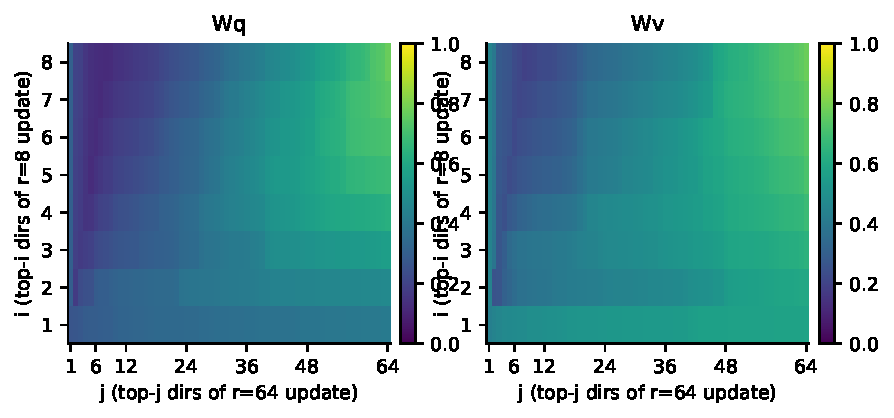
\includegraphics[width=0.9\textwidth]{figures/fig_subspace.pdf}
\caption{$r=8$ 与 $r=64$ 的 LoRA 更新在 $\Delta W_q$ 与 $\Delta W_v$ 上的子空间相似度
（SST-2，第 6 层）。}
\label{fig:subspace}
\end{figure}

\subsection{$\Delta W$ 与 $W$ 的关系}
按论文 Table 7 的方式，把冻结权重 $W$ 投影到 $\Delta W$ 的前 $r$ 个奇异子空间：
$\lVert U^\top W V\rVert_F$，并与随机正交子空间比较。表~\ref{tab:analysis} 给出我们在
SST-2 上训练的 $r=8$ 与 $r=64$ 检查点（第 6 层）的结果；表~\ref{tab:official-proj} 则在
官方 30 轮 MNLI 检查点上重复同样的分析，并对 12 层取平均，用来排除“训练不充分”的解释。

\begin{table}[H]
\centering
\caption{第 6 层冻结权重在 $\Delta W$ 子空间与随机子空间上的投影范数（SST-2 检查点）。}
\label{tab:analysis}
\small
\begin{tabular}{l c c c c c}
\toprule
权重 & 秩 & $\|\Delta W\|_F$ & $\|U^\top W V\|_F$ & 随机子空间 & 放大倍数 \\
\midrule
$W_q$ & 8 & 3.86 & 0.59 & 0.60 & 6.6$\times$ \\
 & 64 & 9.52 & 4.69 & 4.41 & 2.0$\times$ \\
$W_v$ & 8 & 2.53 & 0.50 & 0.42 & 5.0$\times$ \\
 & 64 & 5.72 & 3.17 & 3.24 & 1.8$\times$ \\
\bottomrule
\end{tabular}
\end{table}

\begin{table}[H]
\centering
\caption{官方 RoBERTa-base MNLI LoRA 检查点（$\alpha=16$）上 12 层的平均投影范数。}
\label{tab:official-proj}
\small
\begin{tabular}{l c c c c c c}
\toprule
权重 & $\|W\|_F$ & $\|\Delta W\|_F$ & $\|U^\top W V\|_F$ & $\|U_W^\top W V_W\|_F$ & 随机子空间 & 放大倍数 \\
\midrule
$W_q$ & 55.7 & 10.70 & 1.06 & 18.42 & 0.57 & 11.0$\times$ \\
$W_v$ & 34.6 & 7.31 & 0.58 & 9.53 & 0.35 & 13.1$\times$ \\
\bottomrule
\end{tabular}
\end{table}

三个定性结论与论文一致。第一，$\Delta W$ 子空间上的投影大于随机子空间：官方检查点上
$W_q$、$W_v$ 分别为随机的 \OffProjRatioQ$\times$ 与 \OffProjRatioV$\times$，说明
$\Delta W$ 与 $W$ 的特定方向相关，而不是各向同性的噪声。第二，$\Delta W$ 放大的\emph{不是}
$W$ 的顶部奇异方向：官方检查点第 6 层 $W_q$ 投影到自身前 8 个奇异子空间的范数为
\OffProjWQ，而投影到 $\Delta W$ 子空间只有 \OffProjDWQ（论文对应值 21.67 与 0.32），这与
论文“放大预训练中已学到但未被强调的方向”的解释一致。第三，放大倍数
$\lVert\Delta W\rVert_F/\lVert U^\top W V\rVert_F$ 在官方检查点上平均为
\OffProjAmpQ$\times$（$W_q$）与 \OffProjAmpV$\times$（$W_v$）。

但我们自己的 SST-2 检查点效应弱得多：$r=8$ 时 $W_q$ 的投影仅为随机子空间的 0.98 倍
（$W_v$ 为 1.20 倍），放大倍数为 \AmpQ$\times$ 与 \AmpV$\times$；$r=64$ 时放大倍数降到
\AmpQB$\times$ 与 \AmpVB$\times$。$r=64$ 的这个数值与论文附录 H.4 报告的“$r=64$ 时放大
倍数只有约 2”高度吻合，说明趋势可以复现；但 $r=8$ 的弱相关（0.98 倍）与论文 GPT-3 的
16 倍差距很大。需要注意几个不可比因素：我们的 SST-2 检查点只训练 3 轮（论文的 GPT-3
实验训练 2 轮，但模型参数量大约是我们的三个数量级）；官方 30 轮 MNLI 检查点在同样分析下就达到了
\OffProjRatioQ$\times$ 与 \OffProjAmpQ$\times$，明显强于 3 轮 SST-2 检查点。因此我们倾向
于认为：现象本身（$\Delta W$ 与 $W$ 的非随机对齐、且不是 $W$ 的顶部方向）在 RoBERTa-base
上成立，但其\emph{强度}强烈依赖训练程度与模型规模，不能把 GPT-3 的 21.5 倍直接外推到
小模型。

\section{效率分析}
\label{sec:efficiency}
\subsection{推理时延}
表~\ref{tab:efficiency} 在 RoBERTa-base 上测量单次前向的时延（每个设置交替测量 5 轮、
每轮 20 次前向，取中位数，以抵消 GPU 时钟漂移）。未合并时 LoRA 需要额外计算两个小矩阵
乘法：batch 1 下的开销约 39--40\%（8.75 $\to$ 12.26 ms），batch 32 时降到约 6\%
（63.9 $\to$ 67.8 ms），因为小矩阵乘法被更大的 GEMM 摊薄。合并后三种设置的差异都在
$\pm1\%$ 以内，验证了“零推理时延”的主张。注意这一结论依赖于把 $BA$ 合并进 $W_0$；
若需要在同一个 batch 中动态切换不同任务的 LoRA，则无法预先合并，此时会有上述额外计算。

\begin{table}[H]
\centering
\caption{RoBERTa-base 单次前向时延（每个设置交替测量 5 轮、每轮 20 次前向，取中位数）。}
\label{tab:efficiency}
\small
\begin{tabular}{l c c c c}
\toprule
设置 & Base (ms) & LoRA 未合并 (ms) & LoRA 已合并 (ms) & 开销 \\
\midrule
b1, l32 & 8.75 & 12.26 & 8.82 & +40\% / +1\% \\
b1, l128 & 9.07 & 12.65 & 9.01 & +39\% / -1\% \\
b32, l128 & 63.90 & 67.78 & 63.57 & +6\% / -1\% \\
\bottomrule
\end{tabular}
\end{table}

\subsection{训练显存与速度}
在 RoBERTa-base、batch 16、序列长度 256、FP16 下，LoRA（$r=8$，Q/V）单个训练步的
峰值显存为 \LoraPeakMem{} MB，全量微调为 \FtPeakMem{} MB；单步耗时分别为
\LoraStepMs{} ms 与 \FtStepMs{} ms。LoRA 的显存优势来自不为冻结参数保存 Adam 的一阶、
二阶矩；在本设置下约为全量微调的 \LoraMemPct\%。
这与论文所述“使用自适应优化器时最多降低约 2/3 显存”的方向一致（具体比例取决于模型
大小、batch 与序列长度）。

\section{讨论与结论}
\label{sec:conclusion}

\paragraph{复现到什么程度。}
在方法层面，我们完整复现了 LoRA 的数学形式、初始化、缩放、GPT-2 分组注入与权重合并，
并用单元测试和官方检查点做了交叉验证。在效果层面，受算力限制，我们没有逐字复刻论文的
训练预算，而是保持\emph{方法配置}（数据、模型、学习率、批大小、秩、$\alpha$）不变，
缩减训练轮数。结果是：GLUE 平均 \GlueOursAvg{}（论文 \GluePaperAvg{}），E2E 的 BLEU
\EtwoLoraBleu{}（论文 70.4）；若改用论文的 MNLI 初始化协议，RTE/MRPC/STS-B 分别达到
\InitRteOff{}/\InitMrpcOff{}/\InitStsbOff{}，与论文几乎一致。消融实验与低秩分析在定性上
复现了论文的核心结论。

\paragraph{偏差的来源。}
\begin{enumerate}
  \item \textbf{训练轮数}：MNLI/QQP 等大任务只跑了论文的 1/10 左右，模型尚未收敛；
  \item \textbf{MNLI 初始化协议}：论文对 MRPC/RTE/STS-B 使用 MNLI 适配后的初始化，
        主表未复刻，导致 RTE 明显偏低；\S\ref{sec:mnli-init} 的对照实验证实了该因素的影响
        （官方初始化后 RTE、MRPC、STS-B 分别为 \InitRteOff{}、\InitMrpcOff{}、
        \InitStsbOff{}）；
  \item \textbf{单种子}：论文报告 5 个种子的中位数，单次运行的方差（尤其 RTE/MRPC）不可忽略；
  \item \textbf{实现细节}：E2E 的分词、序列长度与解码流程与官方自定义实现不同。
\end{enumerate}

\paragraph{结论。}
本次复现支持论文的主要结论：LoRA 以约 $10^{-3}$ 量级的可训练参数，在 NLU 与 NLG 任务上
达到与全量微调相当的效果；极小的秩已经足够；固定预算下组合适配优于只适配 $W_q$ 或
$W_k$；合并后不引入推理时延。同时也说明，论文在 GLUE 小任务上的高分依赖较长的训练与
MNLI 初始化，脱离这些设置直接比较绝对值会低估复现难度；低秩分析的效应强度也明显依赖
模型规模与训练程度。

\appendix
\section{复现命令}
\begin{lstlisting}
# 所有实验均在 conda 环境 learn 中运行；离线数据缓存
export HF_HUB_OFFLINE=1 HF_DATASETS_OFFLINE=1 TOKENIZERS_PARALLELISM=false

# GLUE 主实验（以 SST-2 为例；其余任务按表 2 的批大小/学习率/轮数替换）
python src/train_glue.py --task sst2 --method lora --rank 8 --alpha 8 \
  --epochs 10 --batch_size 16 --lr 5e-4 --max_len 256

# 全量微调基线（采用全量微调的标准学习率）
python src/train_glue.py --task sst2 --method ft --epochs 3 \
  --batch_size 32 --lr 2e-5 --max_len 256 --tag ft_sst2

# 秩 / 适配权重消融（3 轮、匹配参数预算）
python src/train_glue.py --task sst2 --method lora --rank 64 --alpha 64 \
  --epochs 3 --batch_size 32 --lr 4e-4 --tag abl_rank64_sst2
python src/train_glue.py --task sst2 --method lora --rank 2 --alpha 2 \
  --targets qkvo --epochs 3 --batch_size 32 --lr 4e-4 \
  --tag abl_tgt_qkvo_r2_sst2

# MNLI 初始化对照（官方检查点，alpha=16）
python src/train_glue.py --task rte --method lora --rank 8 --alpha 16 \
  --epochs 20 --batch_size 32 --lr 5e-4 --max_len 256 --tag initoff_rte \
  --init_lora official/LoRA/examples/NLU/roberta_base_lora_mnli.bin

# GPT-2 medium E2E（训练后自动 beam search 生成并计算多参考指标）
python src/train_e2e.py --method lora --rank 4 --alpha 32 --epochs 5 \
  --batch_size 8 --lr 2e-4 --tag e2e_lora_r4
# 对已有 predictions.txt 按 MR 聚合参考并重新评分
python src/eval_e2e.py --run results/e2e/e2e_lora_r4

# 分析与作图
python src/efficiency.py
python src/subspace.py --ckpt_a results/glue/abl_rank8_sst2/best_lora.pt --rank_a 8 \
  --ckpt_b results/glue/abl_rank64_sst2/best_lora.pt --rank_b 64 --layer 6
python src/make_tables.py && python src/make_figures.py
\end{lstlisting}

\section{产物清单}
\begin{itemize}
  \item \texttt{src/}：全部实现与实验脚本；
  \item \texttt{official/LoRA/}：官方仓库（只读参考）；
  \item \texttt{results/}：每个运行的 \texttt{result.json}、LoRA 权重与预测；
  \item \texttt{logs/}：完整训练日志；
  \item \texttt{report/}：本报告 LaTeX 源码、自动生成的表格与图；
  \item \texttt{data/e2e/}：E2E 原始 CSV。
\end{itemize}

\end{document}
